\chapter{Game Analysis}

In this chapter, I will describe Sagrada from a game-theoretic perspective. 


\begin{description}
    \item[Asymmetric] In asymmetric games, players may have different strategies and payoffs. In Sagrada, this occurs by each player having
    a different Private Objective Card that way receiving extra points for different colored dice.
    
    \item[Non-Zero-Sum] Non-zero-sum games can have outcomes where all players benefit (or lose) from their decisions. On the other hand, Sagrada
    has competitive elements similar to Zero-Sum games e.g. players might sometimes choose dice more to deny others than to benefit their window.
    
    \item[Finite Game with Known Horizon] A game that ends after a predetermined number of moves is considered to have a finite horizon. In the two-player 
    variant of the game, the game ends after a fixed number of 20 moves by every player taking two turns in each of the 10 rounds.
    
    \item[Information Structure] The game features imperfect information due to hidden private objectives and stochastic information represented by future dice rolls.
    
    \item[Dynamic Aspects] Players make decisions one after another, allowing for a reaction to the preceding move.
\end{description}


\section{Branching Factor}

The \textbf{branching factor} defines the number of possible actions available to the agent at 
each decision point within a search tree. Understanding its importance is paramount, as it extremely influences the computational complexity, efficiency, 
and effectiveness of various search-based algorithms. A higher branching factor exponentially increases the number of possible paths within the search tree.

In search-based algorithms such as minimax and MCTS, the branching factor profoundly impacts the efficiency of the search process. A lower branching factor 
typically leads to more efficient exploration of the search space, as the algorithm can delve deeper into the tree without sacrificing computational resources. 
Conversely, a higher branching factor necessitates shallower search depths or more aggressive pruning strategies to maintain acceptable performance levels.

The branching factor varies throughout the game, influenced by factors such as the stage of the game and the presence of 
different types of tool cards. Some tool cards provide players with straightforward actions, resulting in a consistent 
branching factor of one for each use. In contrast, other tool cards introduce variability in branching factor, as their effects 
may differ based on the current state of the game or player choices. For example, tool cards that allow players to relocate dice 
on a board can dramatically increase the branching factor by introducing a huge amount of possibilities.

I will now introduce two basic AI agents: the Random agent, which chooses moves randomly, and the First agent, selecting the first possible move at each decision point.
The first possible move of the player is determined by the order described in the \texttt{Game::possible\_moves()} in Section \ref{principle:possible_moves} .
The following figure illustrates the average branching factor over 1000 games of the Random and First agents across the rounds of the game.


\begin{figure}[H]
    \caption{ Branching factor across the rounds for Random and First agents}
    \centerline{\mbox{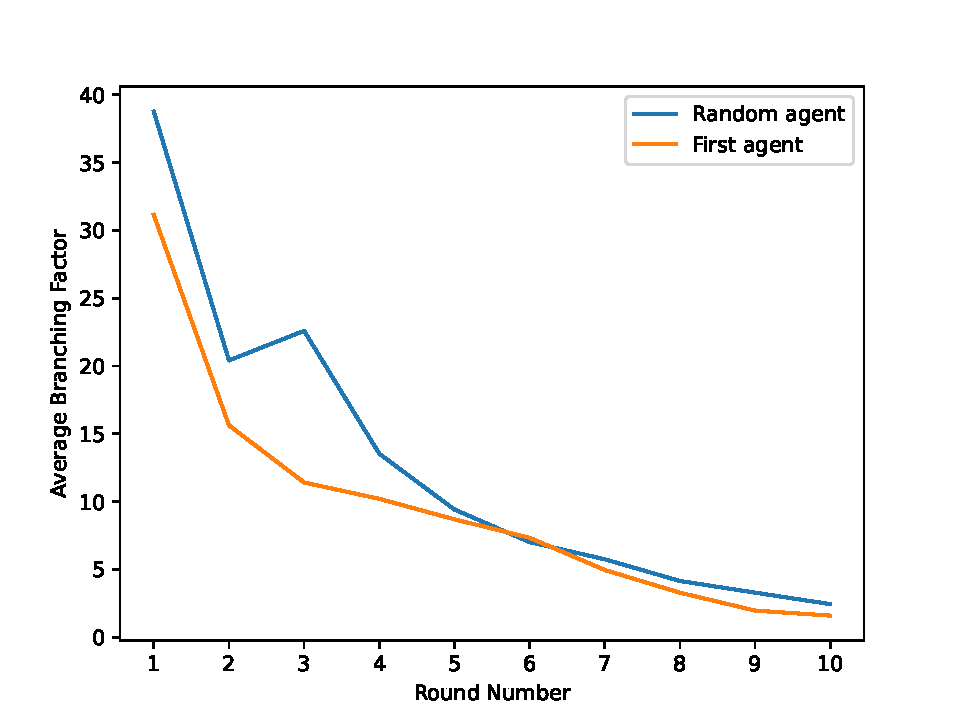
\includegraphics[width=150mm]{img/random_agents_branching_factor.pdf}}}
    \label{fig:example}
\end{figure}


\subsection{Smarter players} \label{subsec:smarter_player_branching_factor}
While these two agents provide a baseline understanding of the branching factor in the game, it's crucial to acknowledge that more strategic or skilled players 
will exhibit different branching factors. Smarter players tend to explore deeper and more selectively within the game tree, leading to a narrower but more focused 
set of potential moves. % An explanation for this phenomenon is that smarter players choose moves that produce uncompletable fields rarely.     
